\clearpage
\section{Modemy v systémech datové komunikace}
\subsection{Jaké jsou základní části modemu? Odůvodněte jejich použití.}

\subsection{Na jaké základní dvě skupiny dle použitého kmitočtového pásma lze rozdělit měniče
signálu? Vysvětlete pojmy linkový kód, klíčování a modulace, přidružte je výše
dotazovaným skupinám.}

\subsection{Co je to skrambler a k čemu slouží?}

\subsection{K čemu slouží linkové kódy? Jaké jsou základní důvody jejich použití? Uveďte příklady
linkových kódů a technologie, kde se využívají.}

\subsection{Uveďte a popište základní typy klíčování? Uveďte vícestavové klíčovací metody.}
Pozn. \textbf{Skrambler} umožňuje odstranění periodicit a dlouhých sekvencí stejných prvků. Přenos v \textbf{základním pásmu} se realizuje pomocí \textbf{linkových kódů}. Linkové kódování definuje realizace signálových prvků tak, aby byla zejména potlačena stejnosměrná složka.
\begin{itemize}
    \item Při přenosu dat v přeloženém pásmu se používá \textbf{modulační} proces, který nazýváme \textbf{klíčování}
    \item Základní typy klíčování: Amplitudové klíčování (ASK), Fázové klíčování (PSK), Kmitočtové klíčování (FSK).
    \item \textbf{Amplitudové klíčování} lze realizovat pomocí násobičky. Vynásobením nosného signálu datového signálu vznikne amplitudově klíčovaný signál. 
    \item \textbf{Kmitočtové klíčování} lze realizovat přepínáním dvojice oscilátorů nosných signálů s užitím násobičky.
    \item \textbf{PSK} je dvojstavové fázové klíčování. Klíčování je opět realizováno pomocí násobičky, na kterou je přivedena nosná a bipolární datový signál .
\end{itemize}
Čtyřstavové fázové klíčování (QPSK), Osmistavové fázové klíčování (8 - PSK)

\subsection{Vysvětlete princip QAM modulace. O jaký typ klíčování se jedná? Co je to IQ modulátor, zakreslete obrázek. Co je to konstelační diagram? }
\begin{itemize}
    \item V bloku OSMS je datový tok rozdělen na dva o shodné přenosové rychlosti.  Vzniklá dvojice signálů je vstupem IQ modulátoru. Číslice před zkratkou QAM uvádí počet stavů.
    \item Kvadraturní amplitudová modulace (QAM) reprezentuje vícestavové kombinované ASK-PSK klíčování.
    \item Protože jeden signál je ve fázi a druhý o pí/2 posunut, označují se tato dvojice jako \textbf{IQ modulátor}.
    
    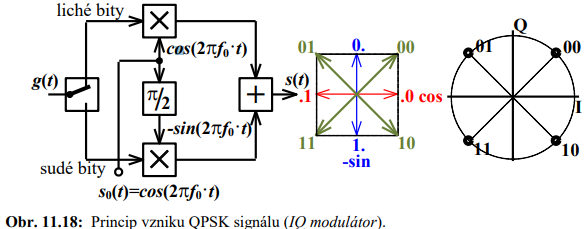
\includegraphics[]{images/image1.png}
    
    \item Fázové klíčování, ale především QAM, se zobrazují s pomocí tzv. \textbf{Konstelačního diagramu}. Diagram uvádí v IQ rovině přiřazení binárních kombinací fázorům nosného signálu.
\end{itemize}

\subsection{Modulace v pojetí protichybového sytému. Co je to eukleidovská vzdálenost? Popište
TCM modulaci?}

\subsection{Vysvětlete princip vícetónových modulací DMT/OFDM. Nakreslete obrázek realizace.}
\begin{itemize}
    \item Hledání metod dalšího zefektivnění datového přenosu vedlo k vícetónovým modulačním metodám.
    \item Můžeme se setkat s \textbf{Diskrétní vícetónovou modulací DMT}, která se uplatňuje zejména na telefonních přípojkách v ADSL a VDSL  
    \item a \textbf{Ortogonálním kmitočtově děleným multiplexem OFDM}, který se uplatňuje na sdílených médiích v technologiích PLC, WLAN, DVB-T. 
    \item Výsledkem aplikace IFFT je 2N komplexních hodnot. Ty jsou vstupem IQ modulátoru, který může být realizován s ohledem na cílové kmitočtové pásmo číslicově nebo analogově
\end{itemize}
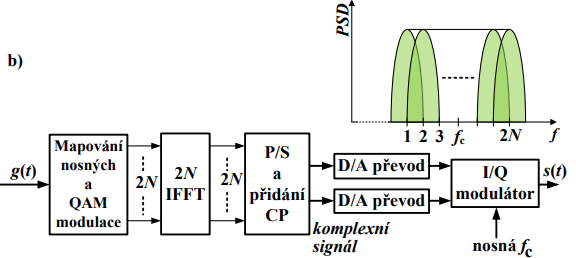
\includegraphics[]{images/image.png}
    
\subsection{Vysvětlete problematiku korekce přenosových charakteristik. Jaké typy ekvalizérů znáte?}

\subsection{Vysvětlete možnosti realizace duplexního přenosu. Co je to vidlice? Vysvětlete princip
vzniku a potlačení ozvěnového signálu.}
